% ===================================================================
%  第 1 节 有限群及其表示（Finite groups and their representations）
%  原文：TASI10.tex 第 299--606 行（PDF p.6--14）
% ===================================================================
\section{有限群及其表示}

\begin{keytakeaways}
  \item 核心对象：有限群及其共轭类、正规子群、商群与群扩张；24 维偶、幺模、正定格恰有 24 个——无根向量的 Leech 格与 23 个 Niemeier 格，其自同构商 $G_N=\Aut(N)/{\rm Weyl}(N)$ \eq{def:niemeier_grp} 给出 Conway 群 $\Co_0$、$M_{24}$、$2.M_{12}$ 等散在单群。
  \item 分类结论：有限单群分为素数阶循环群 $\ZZ_p$、交错群 $\mathcal{A}_n$（$n\geq5$）、16 族 Lie 型群与 26 个散在群；最大的散在群是阶约为 $8\times10^{53}$ 的魔群 $\mathbb M$。
  \item 数学工具：根系统、ADE Dynkin 图（节点连线数 $N_{ij}\in\lbrace0,1,2,3\rbrace$）、最高根与 Coxeter 数；格的正定、整、偶、幺模性质，以及对偶格与根向量。
  \item 表示论结果：Maschke 定理保证有限群的复表示完全可约；特征标正交关系 \eq{eq:orthog_char} 推出不等价不可约表示的个数等于共轭类的个数，全部表示数据可压缩为一张 $\Cl(G)\times\Cl(G)$ 的特征标表。
  \item 后续常用工具：特征标表上的幂映射、置换表示的轮换型（cycle shape）与 frame shape；射影表示与 Schur 乘子在处理中心扩张时不可或缺。
\end{keytakeaways}

本节简要回顾有限群及其表示的基本概念，主要依照 \cite{HamermeshMorton1962Gtai,JonesH.F.HughF.1998Grap,webb_2016}（另见 \cite{2009arXiv0901.0827E}）。

\subsection{群}
\label{subsec:Groups}

群是一个集合 $G$，连同一种“乘法”运算 $\bcdot:G\times G\rightarrow G$，形式上记作 $(G,\bcdot)$。这个运算的符号通常省略不写，我们常把 $a\bcdot b$ 写成 $ab$。群必须满足以下公理：
\begin{enumerate}
\item \textbf{封闭性：} 对任意 $a,b\in G$，有 $ab=c\in G$。
\item \textbf{结合律：} 对任意 $a,b,c\in G$，有 $(ab)c=a(bc)$。
\item \textbf{单位元：} 存在唯一的单位元 $e\in G$，使得对任意 $g\in G$ 有 $eg=ge=g$。
\item \textbf{逆元：} 对每个 $g\in G$，存在唯一的逆元 $g^{-1}\in G$，使得 $gg^{-1}=g^{-1}g=e$。此外还有 $e^{-1}=e$。
\end{enumerate}

% [Tutor Note: 公理中的“唯一”其实不必单列：若 $e,e'$ 都是单位元，则 $e=ee'=e'$；逆元同理。注意元素的阶 $|g|$ 是使 $g^{|g|}=e$ 的最小正整数，不是“任意满足的指数”，阶为 1 的元素只有单位元；$|g|=\infty$ 指不存在这样的正整数。]

注意，一般情形下 $ab\neq ba$。若对每个 $a,b\in G$ 都有 $ab=ba$，即群运算可交换，则称该群为\emph{阿贝尔}（Abelian）群。$G$ 中元素的个数称为 $G$ 的\emph{阶}，它可以是有限的，也可以是无限的。我们还定义\emph{元素的阶} $|g|$ 为：把 $g$ 与自身相乘、直到首次得到单位元所需的次数，即 $g^{|g|}=e$（阶也可以是无限的）。

~\\
下面我们简要总结群论中的几个重要概念。

\myparagraph{群同态。}
设 $(G,\bcdot)$ 与 $(F,\star)$ 是两个群。若映射 $\phi:G\rightarrow F$ 保持 $G$ 的群结构，则称它为\emph{群同态}。换言之，$\phi$ 必须满足
\begin{equation}
\phi(a\bcdot b)=\phi(a)\star\phi(b)~,
\end{equation}
对任意 $a,b\in G$ 成立。若还存在逆同态映射 $\phi^{-1}:F\rightarrow G$，则 $G$ 与 $F$ 同构；这样的两个群抽象地说是同一个群，但它们的实现可以不同。同构 $G\rightarrow G$ 称为\emph{自同构}，也常称为 $G$ 的对称性。$G$ 的全部自同构构成的集合记作 $\Aut G$，它本身构成一个群。

\myparagraph{共轭类。}
若存在元素 $g\in G$ 使 $gag^{-1}=b$，则称群元素 $a,b\in G$ 彼此共轭。此时我们按惯例记作 $a\sim b$。共轭是一种等价关系，因为它自反（$a\sim a$）、对称（$a\sim b$ 当且仅当 $b\sim a$）且传递（若 $a\sim b$ 且 $b\sim c$，则 $a\sim c$）。这一关系把 $G$ 分成互不相交的子集 $[a]\subset G$，称为\emph{共轭类}，每个类包含所有彼此共轭的元素：
\begin{equation}
[a]=\left\lbrace b\in G~|~gag^{-1}=b\text{~~对某个~~}g\in G\right\rbrace~.
\end{equation}
显然，共轭类可由其中任一元素代表，即对所有 $b\sim a$ 有 $[a]=[b]$。不同共轭类的个数称为 $G$ 的\emph{类数}，这里记作 $\Cl(G)$。同一个类的所有元素都有相同的阶。容易看出，若一个元素与群中所有其他元素都可交换，则它自成一个共轭类。于是，在阿贝尔群中每个类只含一个元素，类数等于群的阶。

% [Tutor Note: 下文定义陪集时会再出现一个等价关系 $a\sim b\iff ah=b$（对某个 $h\in H$），它与这里的共轭关系 $gag^{-1}=b$ 是两回事，原文特意提醒“勿混淆”。另外类数记号是正体 $\Cl(G)$，与 Conway 群 $\Co_0$ 的 Co 无关。]

共轭类的常用记号是写出其元素的阶，再跟一个字母。例如 $4A$ 表示一个阶为四的类，$4B$ 表示另一个阶为四的类，$6A$ 表示一个阶为六的类，依此类推。单位元总是自成一类，即 $1A$，它是唯一阶为一的类。

\myparagraph{子群。}
子群 $H$ 是子集 $H\subset G$，它本身在从 $G$ 继承的群结构下构成群。注意单位元 $e$ 总构成一个阶为 1 的子群 $\lbrace e\rbrace$，称为平凡子群。除平凡子群与 $G$ 自身之外的子群称为 $G$ 的\emph{真子群}，记作 $H<G$（若允许 $H=G$，我们用 $H\leq G$）。

\emph{正规子群} $N$ 也记作 $N\triangleleft G$，是 $G$ 中在所有元素共轭作用下都不变的子群：
\begin{equation}
N\triangleleft G~\Leftrightarrow~gNg^{-1}=N\text{ 对任意 }g\in G~.
\end{equation}
因此，$N$ 必然是若干共轭类的并。$G$ 的\emph{极大正规子群}是指不被 $G$ 的任何其他正规子群（$G$ 自身除外）包含的正规子群。正规子群在商群与群扩张中起突出作用（见下文）。

群 $G$ 的\emph{中心} $Z(G)$ 是与所有其他元素都可交换的元素的集合，即
\begin{equation}
Z(G):=\lbrace a\in G\,\lvert\, ab=ba\text{~~对任意 } b\in G\rbrace~.
\end{equation}
中心总是 $G$ 的正规子群。元素 $g\in G$ 的\emph{中心化子}（centralizer）类似地定义为
\begin{equation}
C_G(g)=\lbrace a\in G\,\lvert\, ag=ga\rbrace,~
\end{equation}
即所有与 $g$ 可交换的元素构成的集合。显然，元素的中心化子总是 $G$ 的子群。

\myparagraph{陪集。}
设 $H$ 是 $G$ 的子群，取 $g\in G$。我们定义 $H$ 在 $G$ 中关于 $g$ 的\emph{左陪集}为子集
\begin{equation}
gH=\lbrace gh~|~h\in H\rbrace~.
\end{equation}
$H$ 在 $G$ 中全部左陪集构成的集合记作 $G/H:=\lbrace gH~|~g\in G\rbrace$。类似地，$H$ 在 $G$ 中关于 $g$ 的\emph{右陪集}定义为
\begin{equation}
Hg:=\lbrace hg~|~h\in H\rbrace~,
\end{equation}
而 $H$ 在 $G$ 中全部右陪集构成的集合记作 $H\backslash G:=\lbrace Hg~|~g\in G\rbrace$。

也可以用 $G$ 上的等价关系更直观地定义左陪集（注意不要与共轭混淆）：对 $a,b\in G$，若存在 $h\in H$ 使 $ah=b$，则令 $a\sim b$，即 $a$ 与 $b$ 相差在右侧乘一个 $H$ 中的元素。此时 $a,b$ 代表同一个等价类，恰为陪集 $aH=bH$。所有这样的等价类构成 $G/H$，这是把 $G$ 作为集合的一个互不相交的划分。相应的陈述对右陪集同样成立。关于陪集，有几个有用的事实：
\begin{itemize}
\item 左陪集的个数总等于右陪集的个数，称为 $H$ 在 $G$ 中的\emph{指数}，记作 $[G:H]$。
\item 若 $G$ 是有限群，Lagrange 定理说指数等于 $G$ 的阶除以 $H$ 的阶，即 $[G:H]{|H|}={|G|}$。这刻画了在 $H$ 对应的陪集等价关系下 $G$ 如何被划分。
\item $H$ 的左陪集与右陪集所含元素个数相同，都等于 $H$ 的阶。
\item 正规子群的左陪集与右陪集重合，这由其定义即可看出。
\end{itemize}

% [Tutor Note: Lagrange 定理的公式 $[G:H]{|H|}={|G|}$ 只对有限群成立；对无限群，指数 $[G:H]$ 可以是有限的而 $|H|$、$|G|$ 都无限。另注意 $G/H$ 与 $H\backslash G$ 是方向不同的陪集集合，只有当 $H$ 正规时二者才作为群同构。]

\myparagraph{商群与群扩张。}
陪集和共轭类一样，一般不是子群。不过，给定正规子群 $N$，右陪集的集合 $G/N$（与左陪集集合重合）继承 $G$ 的群结构，称为\emph{商群}。这可由 $(aN)(bN) = (ab)N$ 看出。于是正规子群 $N$ 可看作同态 $\psi:G\rightarrow G/N$ 的核。注意，一般 $G/N$ 不同构于 $G$ 的任何子群。此外，$G/N$ 的阶等于指数 $[G:N]=|G|/|N|$。

现在考虑群的\emph{短正合列}
\begin{equation}
1\rightarrow M\xrightarrow{\phi} G\xrightarrow{\psi} Q\rightarrow1~. 
\end{equation}
这表示：$M$ 通过 $\phi$ 在 $G$ 中的嵌入 $\phi(M)$ 是同态 $\psi$ 的核；换言之，$M$ 同构于正规子群 $N\triangleleft G$，且 $Q\cong G/N$。此时称 $G$ 是 $Q$ 关于 $M$ 的一个\emph{扩张}。若存在同态（嵌入）$\widetilde{\psi}:Q\rightarrow G$ 使得 $\psi\circ \widetilde{\psi}=\text{id}_Q$（$Q$ 上的恒等映射），则称该扩张及相应的序列是\emph{分裂}的。我们用半直积表示这种分裂扩张，$G=N\rtimes Q$。否则，扩张称为\emph{非分裂}的，记作 $G=N.Q$~。

% [Tutor Note: 分裂同态 $\widetilde{\psi}$ 不是任意的：它给出 $Q$ 在 $\Aut(N)$ 上的作用，从而决定半直积的结构。同样的 $N$、$Q$ 可给出不同的半直积，例如 $S_3=\ZZ_3\rtimes\ZZ_2$ 中作用非平凡；若 $|N|$ 与 $|Q|$ 互素，Schur–Zassenhaus 定理保证任何扩张都分裂。]

\subsection{有限群的分类}

从现在起我们只讨论有限群，即元素个数有限的群。有限群的分类问题可以化归为有限单群的分类。若一个群没有真正规子群，则称它为\emph{单群}。若 $G$ 不是单群，则总可以通过取极大正规子群的商，把 $G$ “分解”为一列更小的群。确切地说，可以考虑\emph{合成列}，其形式为
\begin{equation}
1\triangleleft N_1\triangleleft N_2\triangleleft\cdots \triangleleft N_{n-1}\triangleleft N_n=G~.
\end{equation}
这里 $1$ 表示平凡群，合成列的每一步涉及 $N_i$ 的极大正规子群 $N_{i-1}$ 以及相应的商群 $N_i/N_{i-1}$。可以证明，所得商群都是单群；Jordan--H{\"o}lder 定理保证：对给定的 $G$，两个不同的合成列给出相同的单群。因此，研究有限单群在很大程度上足以理解一般有限群。

经过半个多世纪的努力、逾百位数学家的参与，以及多达数万页的证明，全部有限单群已经分类（历史评述见 \cite{GorensteinDaniel1982Fsg:, RonaldSolomon2001Abho}）。它们属于以下四类之一：素数 $p$ 对应的循环群 $\ZZ_p$、交错群 $\mathcal{A}_n$（$n\geq5$）、16 族 Lie 型群，以及 26 个\emph{散在群}。与其余有限单群不同，26 个散在群“零星”出现，不属于任何无限族。我们将在下一小节进一步讨论散在群。

% [Tutor Note: 有限单群分类定理（CFSG）1955 年起步、1983 年宣布完成，2004 年 Aschbacher–Smith 补上 quasithin 情形后才算完整，“逾万页”仍是保守说法。四类中循环群与交错群各是无限族，Lie 型群共 16 族（含例外型与扭转型），散在群只有 26 个；而 $\mathcal{A}_5$ 是最小的非阿贝尔单群，阶为 60。]

\subsection{散在群与格}
\label{sec:sporadic_lattices}

最大的散在群是 Fischer–Griess 魔群 $\mathbb M$，它的名称来自其巨大的规模。它的元素个数为
\[
|\mathbb M| =  2^{46} \cdot 3^{20} \cdot 5^9 \cdot 7^6 \cdot 11^2 \cdot 13^3 \cdot 17 \cdot 19 \cdot 23 \cdot 29 \cdot 31 \cdot 41 \cdot 47 \cdot 59 \cdot 71 \approx 8 \times 10^{53}~, 
\]
这大致相当于太阳系中原子的数目。魔群包含 26 个散在群中的 20 个，作为其子群或子群的商；Robert Griess 称这 20 个群构成一个\emph{happy family}（快乐家族）的 3 代。具体地说，happy family 包含五个 Mathieu 群 $M_{11}, M_{12}, M_{22}, M_{23}, M_{24}$。它们都是 $M_{24}$ 的子群，而 $M_{24}$ 又是置换群 $S_{24}$ 的子群；它们也是最早被发现的散在群。其余 6 个与魔群无关的群称为散在群的 \emph{pariah} 群。

散在群的“散在”本性使其存在多少有些神秘，人们不禁要问：它们的“自然”表示是什么？一个重要提示是：许多散在群，尤其是与魔群相关的那些，都作为各种特殊格的自同构群之商的子群出现。涉及散在群的月光的出现，为这一问题提供了重要线索；而月光的构造往往依赖这些特殊格的存在。因此，下面我们简要回顾格及其根系统的定义，并介绍与月光相关的特殊格。

设 $V$ 是 $r$ 维实向量空间，配备内积 $\langle\cdot,\cdot\rangle$。若非零向量构成的有限子集 $X\subset V$ 满足以下条件，则称 $X$ 为\emph{秩 $r$ 的根系统}：
% [Tutor Note: 下面第 2 条的 $\a$ 就是 $\alpha$（preamble 中自定义宏 \a 展开为 \alpha），而 $\beta$ 写作 \beta。反射公式 $\beta-2\langle\alpha,\beta\rangle/\langle\alpha,\alpha\rangle\,\alpha$ 是 β 关于垂直于 α 的超平面的反射，第一个 β 不能漏。第 4 条要求 $2\langle\alpha,\beta\rangle/\langle\alpha,\alpha\rangle$ 为整数，这是根系“整性”的根源，也是后面格取整的基础。]
\begin{itemize}
\item $X$ 张成 $V$。
\item $X$ 在反射下封闭。即对任意 $\a, \beta\in X$，有 $\beta-2\dfrac{\langle\alpha,\beta\rangle}{\langle\alpha,\alpha\rangle}\alpha \in X$。
\item 属于 $X$ 的 $\alpha\in X$ 的倍数只有 $\alpha$ 与 $-\alpha$。
\item 对任意 $\alpha,\beta\in X$，有 $\dfrac{2\langle\alpha,\beta\rangle}{\langle\alpha,\alpha\rangle}\in\ZZ$。
\end{itemize}
根系统中的元素 $\alpha\in X$ 称为\emph{根}。若根系统 $X$ 不能分割为两个真正交子集 $X=X_1\cup X_2$，则称它不可约。这样的根系统的根至多有两种可能的长度。若所有根长度相同，则称该不可约根系统为\emph{单边}（simply-laced）。可以选取根的子集 $\Phi$，其元素 $f_i\in X$（$i=1,\dots,r$），使得每个根都能写成 $f_i\in\Phi$ 的整系数线性组合，且系数全为负或全为正。这样的子集称为一组\emph{单根}；在关于所有根的反射所生成的群（称为 $X$ 的\emph{Weyl 群}，记作 Weyl$(X)$）的作用下，单根集唯一（至多相差 Weyl 群的一个作用）。

对每个不可约根系统可附上一个连通的\emph{Dynkin 图}。每个单根对应一个节点；两个不同单根 $f_i,f_j$ 对应的节点之间连 $N_{ij}$ 条线，其中
\begin{equation}
N_{ij}=\frac{2\langle f_i,f_j\rangle}{\langle f_i,f_i\rangle}\frac{2\langle f_j,f_i\rangle}{\langle f_j,f_j\rangle}\in\lbrace0,1,2,3\rbrace~.
\end{equation}
对单边根系统只有 $N_{ij}\in\lbrace0,1\rbrace$。它们对应 $A_n,D_n, E_6, E_7, E_8$ 型 Dynkin 图，下标表示相应根系统的秩，如图 \ref{fig:dynkin} 所示。

\begin{figure}[t]
  \begin{center}
    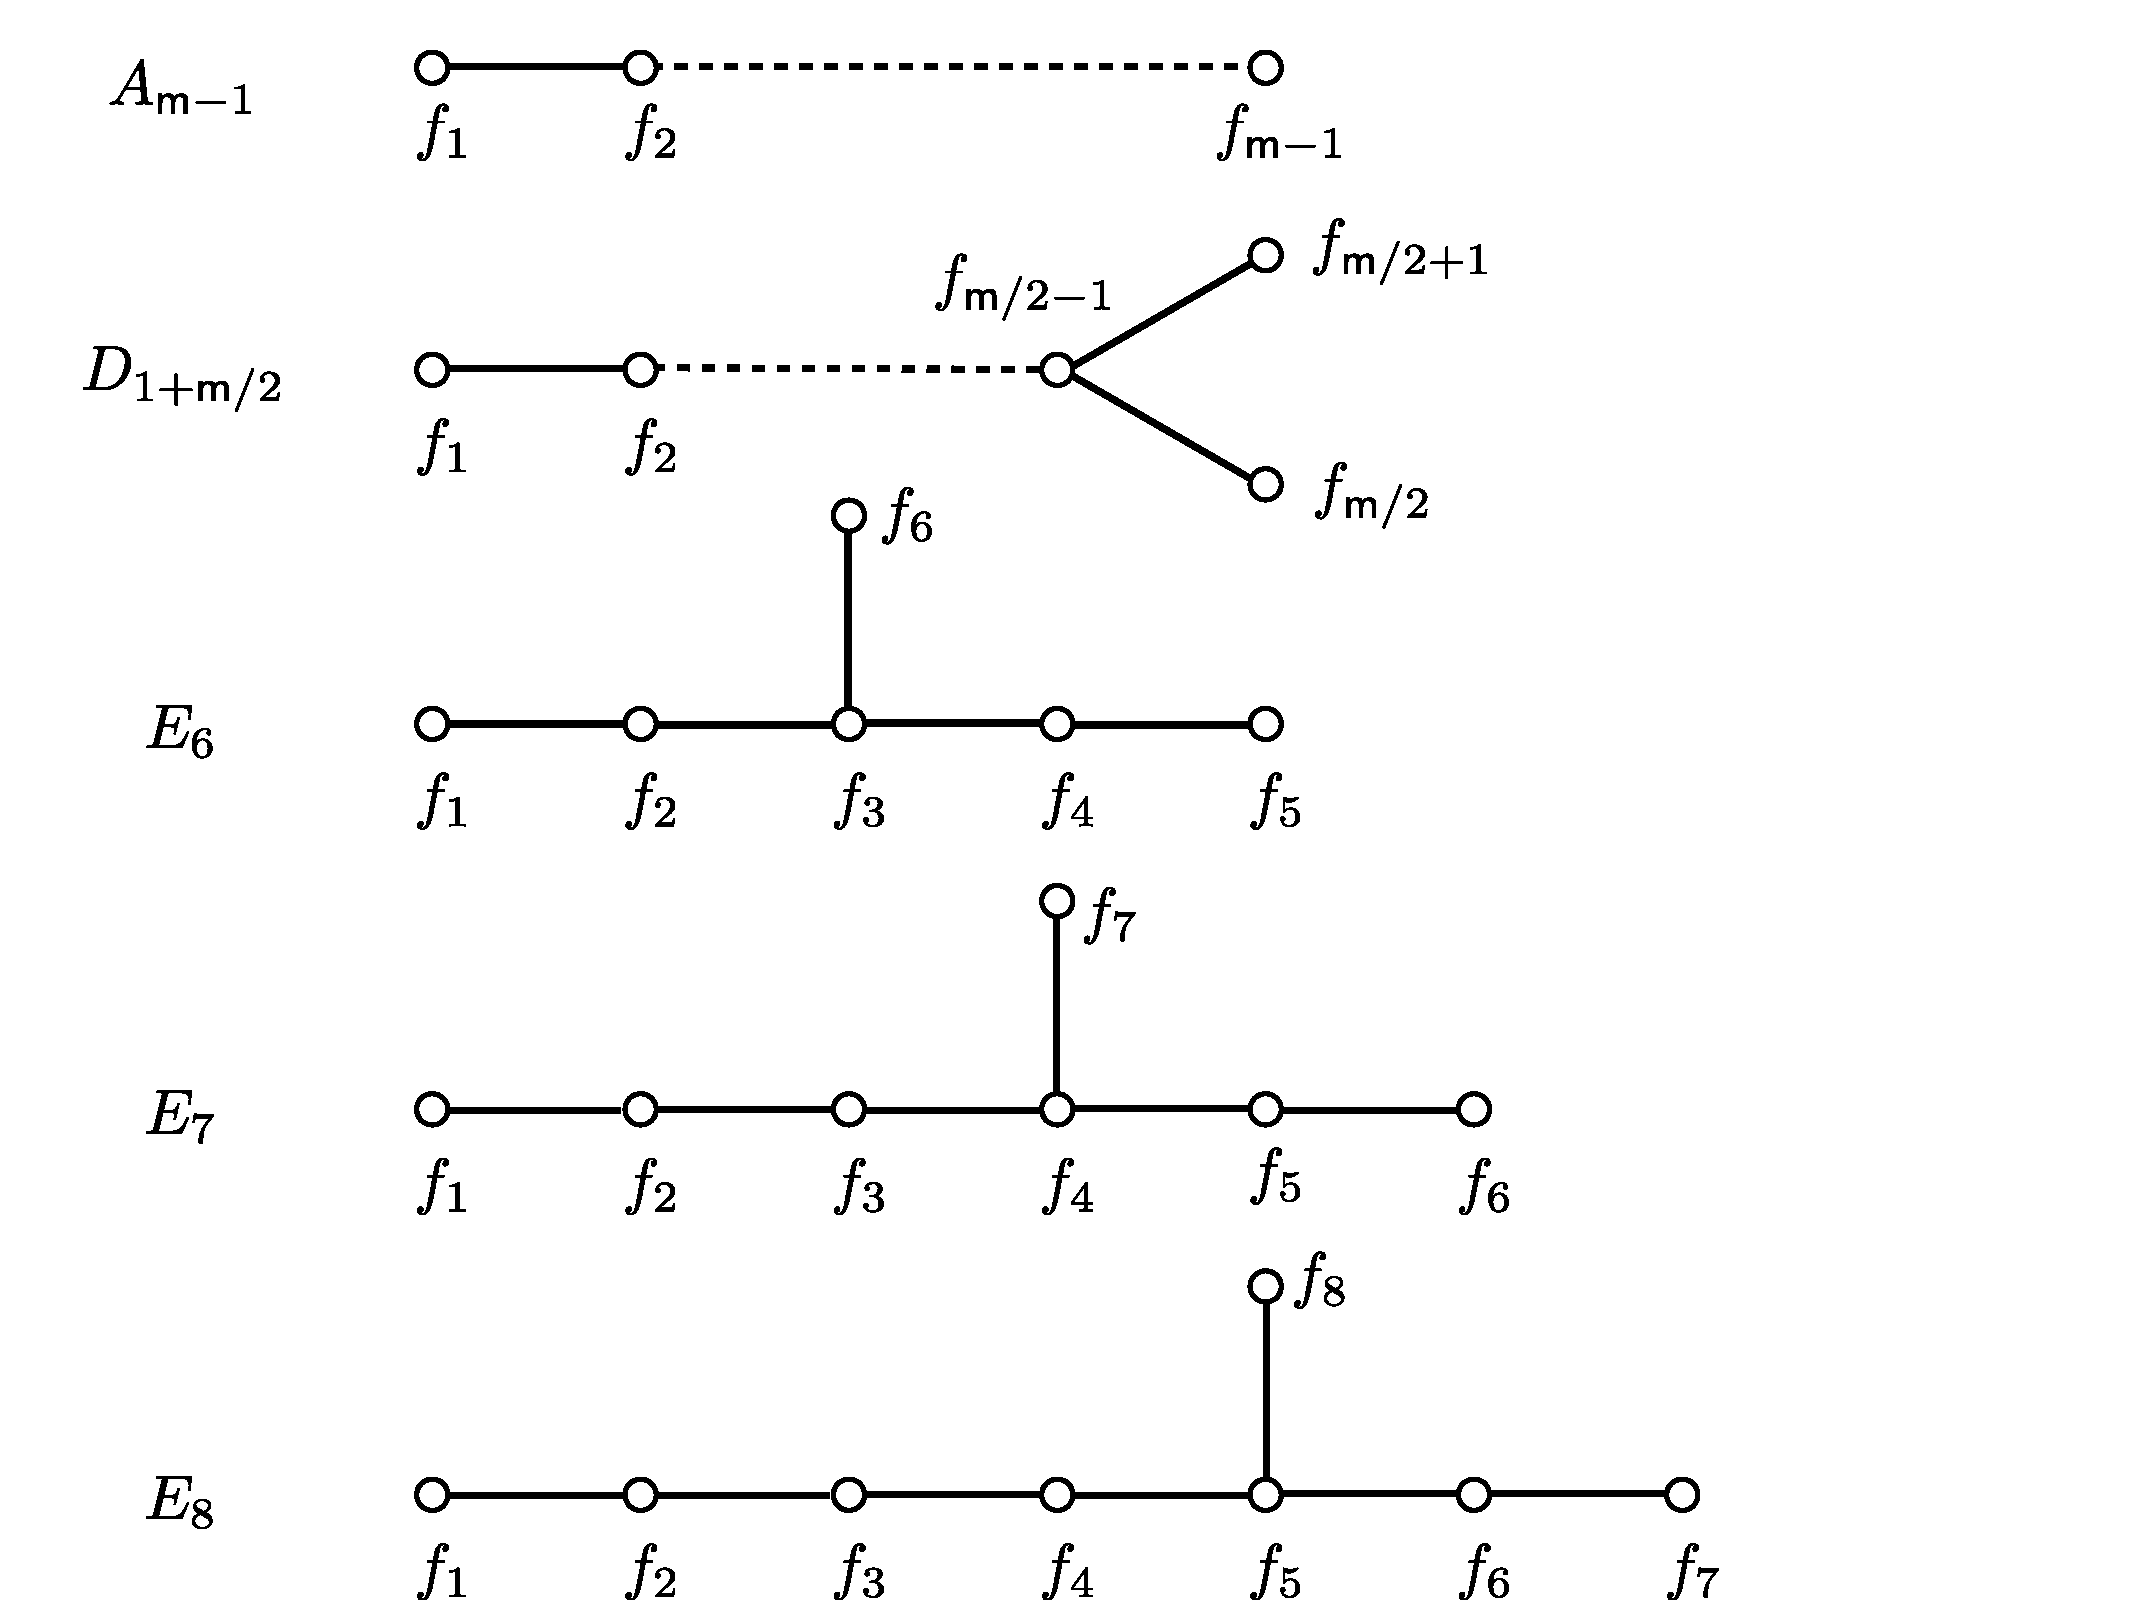
\includegraphics[width=0.62\linewidth]{figures/fig2_ade_dynkin.pdf}
    \caption{ADE Dynkin 图。（原文 p.10，图 1）}
    \label{fig:dynkin}
  \end{center}
\end{figure}

每个不可约根系统相对于给定的单根集 $\Phi$ 含有唯一的\emph{最高根} $\theta$，其分解
\begin{equation}
\theta=\sum_{i=1}^r a_i f_i
\end{equation}
使和 $\sum a_i$ 最大。于是 $X$ 的\emph{Coxeter 数}（Coxeter number）定义为
\begin{equation}
\text{Cox}(X):=1+\sum_{i=1}^ra_i~.
\end{equation}
Coxeter 数也可以用 Weyl$(X)$ 来定义。关于所有单根的反射之积 $w=r_{f_1}r_{f_2}\cdots r_{f_r}\in W^X$ 称为\emph{Coxeter 元}，它的阶等于 Coxeter 数 $m$。

% [Tutor Note: “Coxeter 元的阶等于 Coxeter 数”对不可约根系统成立，原文未给证明，标准论证见 Bourbaki《Lie Groups and Lie Algebras》第 V–VI 章。对单边根系统还有 $\text{Cox}(X)=|X|/r$（根的个数除以秩）：$E_8$ 有 240 个根、秩 8，故 Coxeter 数为 30，可用来快速验算。]

秩为 $n$ 的\emph{格} $L$ 是一个同构于加法群 $\ZZ^n$ 的自由阿贝尔群，配备对称双线性型 $\langle\cdot,\cdot\rangle$。把 $L$ 嵌入 $\RR^n$，就得到向量空间 $\RR^n$ 中一个点集的图像。对我们的用途来说，格的一些有用性质如下：
\begin{itemize}
\item \emph{正定}：双线性型在 $\RR^n$ 上诱导正定内积。
\item \emph{整}：对任意 $\lambda,\mu\in L$，有 $\langle\lambda,\mu\rangle\in\ZZ$。
\item \emph{偶}：对任意 $\lambda\in L$，有 $\langle\lambda,\lambda\rangle\in2\ZZ$。
\item \emph{幺模}：对偶格 $L^*:=\lbrace \lambda\in L \otimes_\ZZ \RR |~\langle\lambda,L\rangle\subset\ZZ\rbrace$ 同构于格本身。
\end{itemize}
$L$ 中满足 $\langle\lambda,\lambda\rangle=2$ 的所有元素 $\lambda\in L$ 称为 $L$ 的\emph{根}。

24 维的偶、幺模、正定格在月光的若干实例中扮演特殊角色，我们将在本讲义的第二部分与第三部分讨论。H. V. Niemeier 于 1973 年证明：这样的格只有 24 个互不等价的 \cite{Nie_DefQdtFrm24}。其中之一由 J. Leech 于 1967 年首次发现，称为\emph{Leech 格}，它是这 24 个格中唯一没有根向量的 \cite{Lee_SphPkgs,Con_ChrLeeLat,Lee_SphPkgHgrSpc}。其余 23 个我们称为 \emph{Niemeier 格}，它们具有非平凡的根系统。事实上，Niemeier 格的一种有用构造是把根格与适当的“粘合向量”（glue vectors）组合起来 \cite{sphere_packing}。结果表明，23 个 Niemeier 格由根系统 $X$ 唯一标记，这些 $X$ 称为 \emph{Niemeier 根系统}；它们恰是满足以下条件的 23 个单边（ADE）根系统之并 $X= \cup_i  Y_i$：1) 所有分量的 Coxeter 数相同，${\rm Cox}(Y_i)={\rm Cox}(Y_j)$；2) 总秩等于格的秩 $\sum_i {\rm rk} (Y_i)=24$。这 23 个之中的例子包括 $24A_1$、$2A_{12}$、$8E_8$ 与 $D_{16}E_8$。

% [Tutor Note: 原文举例作 $8E_8$，但 $8E_8$ 的秩为 $8\times8=64$，与同一句的条件 2（总秩 24）直接矛盾；正确的 Niemeier 根系统应为 $3E_8$（三份 $E_8$，秩 $3\times8=24$）。此处疑为原文笔误，译文照录未改，详见报告。]

对这 24 个秩 24 的偶、幺模、正定格 $N$，各定义一个有限群
\be\label{def:niemeier_grp}
G_{N} := {\rm Aut}(N)/{\rm Weyl } (N), 
\ee
其中 ${\rm Weyl } (N)$ 表示 $N$ 的根系统的 Weyl 群。特别地，当 $N=\Lambda$ 为 Leech 格时，Weyl 群 ${\rm Weyl } (\Lambda)$ 是平凡群，而 $G_{\Lambda} \cong \Co_0$ 就是 Conway 群 $\Co_0$。考虑这一群的商以及稳定各种结构的子群，可以得到许多散在群。例如，散在单群 $\Co_1$ 由对中心的商给出，$\Co_1\cong \Co_0/\{\pm1\}$；Mathieu 群 $M_{23}$ 则作为固定某个秩 2 子格的子群出现。详见 \cite{sphere_packing} 第 10 章。若改取 $N$ 为根系统 $24A_1$ 的 Niemeier 格，则有限群 $G_{N}\cong M_{24}$ 即最大的 Mathieu 群。对根系统 $12A_2$ 的 Niemeier 格，有限群为 $2.M_{12}$，即 Mathieu 群 $M_{12}$ 的非平凡扩张。这些群将在月光中（参见 \S\ref{sec:conway_moonshine}、\S\ref{sec:M24moonshine}、\S\ref{sec:umbral}）以及对其物理背景的讨论中（参见 \S\ref{chap:moonshineK3}）起重要作用。

% [Tutor Note: $G_N=\Aut(N)/\Weyl(N)$ 的取法有讲究：Weyl 群由根反射生成、总含于 $\Aut(N)$，除掉它才能留下在根系统上作用平凡的那部分对称性；Leech 格无根向量、Weyl 群平凡，故 $G_\Lambda=\Co_0$。$24A_1$ 给出 $M_{24}$、$12A_2$ 给出 $2.M_{12}$，说明同一个 Niemeier 格既决定根系统、也决定对应的月光群；Schur 乘子为 2 正是 $M_{12}$ 出现非平凡扩张的原因。]

\subsection{有限群的表示}
\label{subsec:rep}

群的结构正是描述对称性所需要的。要把它用起来，还需要群的表示这一概念。以下我们只讨论\emph{复表示}，即考虑群在复向量空间 $V$ 上的作用。更确切地说，考虑群同态 $\r:G\rightarrow\GL(V)$。我们可以把像 $\r(g)$ 看作可逆的 $n\times n$ 复矩阵。特别地有 $\rr\left(g^{-1}\right)=(\rr(g))^{-1}$。向量空间连同映射 $(V,\rr)$ 称为维数为 $n$ 的\emph{表示}。人们常把 $V$ 或 $\rr$ 单独称为表示，而隐含指整套数据。此时向量空间 $V$ 也称为 $G$-模，并说它带有 $G$-作用。若不存在两个不同元素 $g,g'\in G$ 使得 $\rho(g)=\rho(g')$，则称该 $G$-作用\emph{忠实}（相应的表示也称为忠实的）。

\myparagraph{不可约表示与对偶表示。}
给定两个表示 $(V,\rr)$ 与 $(V',\rr')$，可以直接定义它们的直和与张量积，从而得到新的表示 $V\oplus V'$ 与 $V\otimes V'$。

% [Tutor Note: 张量积 $V\otimes V'$ 的特征标等于两个特征标之积（即下文 (1.17) 的第二个等式），这是“特征标构成交换结合代数”的来源。但若群只以相差一个相位的意义作用（射影表示），$V\otimes V'$ 会把相位（2-上链）暴露出来，必须改用 Schur 乘子与中心扩张处理；本节讨论的都是“真”表示，后文月光模在中心扩张下用到的正是射影表示。]

若存在可逆 $n\times n$ 矩阵 $M$ 使得对任意 $g\in G$ 有 $M\rr'(g)=\rr(g)M$，则称两个表示 $\rr,\rr'$ 等价。表示 $(V,\rr)$ 的\emph{子表示}是一个表示 $(U,\rr')$，其中 $U$ 是子空间 $U\subset V$，在 $G$ 的作用下不变，$\rr'$ 是 $\rr$ 到 $U$ 的限制。若表示 $V$ 不含任何真子表示，则称它\emph{不可约}；若它不能写成两个（或更多）非零子表示的直和，则称它\emph{不可分解}。对有限群，这两个概念一致。若一个表示是有限多个不可约表示的直和，即它可完全分解为不可约的部分，则称它\emph{完全可约}。$G$ 的不可约表示在限制到子群 $H<G$ 时可以变为可约的，它分解为 $H$ 的不可约表示的方式由所谓的\emph{分支规则}（branching rules）给出。

所谓的 Maschke 定理说，有限群的所有（有限维）表示总是完全可约的。证明分两步。首先证明幺正表示总是完全可约的，用到的事实是：给定内积 $\lbrace\cdot,\cdot\rbrace: V\times V \to \CC$，若 $U$ 是 $V$ 的子表示，则 $U$ 在 $V$ 中的正交补也是子表示。接着证明任何表示关于群不变内积
\begin{equation}
\lbrace v,w\rbrace\coloneqq\frac{1}{| G|}\sum_{g\in G}\langle\rr(g)v,\rr(g)w\rangle,~~v,w\in V~,
\end{equation}
都是幺正的，这就完成了证明。

% [Tutor Note: 关键在第 1 步：$U$ 的 $G$-不变正交补之所以存在，靠的是内积群不变；而平均化 $\frac{1}{|G|}\sum_{g\in G}$ 要求 $|G|$ 在基域中可逆，故 Maschke 定理对特征不整除 $|G|$ 的域都成立（这里基域是 $\CC$）。若换成射影表示，平均化只能做到相差 2-上链，完全可约性要另行论证。]

我们还提到表示 $\rr$ 的\emph{对偶表示} $\rr^*$，它定义为
% [Tutor Note: 对偶表示公式里 $g^{-1}$ 与转置缺一不可：若漏掉 $g^{-1}$，则 $\rho^*(gg')$ 与 $\rho^*(g)\rho^*(g')$ 反序，得不到群同态。取 $\rho$ 幺正时 $\rho(g^{-1})=\rho(g)^{\dagger}$，于是 $\rho^*(g)=\overline{\rho(g)}$，这正是“对偶等价于复共轭”的由来；非幺正情形只能说对偶，不能与复共轭混同。]
\begin{equation}
\label{eq:dual_rep}
\rr^*(g):=\left(\rr\left(g^{-1}\right)\right)^T~,~~g\in G~, 
\end{equation}
这是对偶空间 $V^*=\End(V,\CC)$ 上的自然群作用。取 $\rho$ 为幺正表示，则 $\rho^*(g)=\overline{\rho(g)}$。换言之，对偶表示等价于复共轭表示。

\myparagraph{特征标。}
表示 $(V,\rr)$（$V$ 是 $\CC$ 上的向量空间）的\emph{特征标}（character）$\x_\rr$ 是由表示矩阵的迹定义的映射 $G\rightarrow\CC$：
\begin{equation}
\x_\rr(g)\coloneqq\tr(\rr(g))~,~~g\in G.
\end{equation}
我们也常用 $\tr_V g$ 表示这个迹。若 $\rr$ 不可约，则 $\x_\rr$ 称为不可约特征标。有限群特征标的一些性质总结如下：
\begin{itemize}

\item 特征标是\emph{类函数}，即 $\x_\rr\left(hgh^{-1}\right)=\x_\rr(g)~~\forall~g,h\in G$。这直接来自迹的循环性质。

\item 有限群的两个复表示有相同的特征标，当且仅当它们等价；这可用下面讨论的正交性证明。

\item $G$ 的特征标限制到子群 $H<G$ 上，是 $H$ 的特征标。

\item $\x_\rr\left(g^{-1}\right)=\overline{\x_\rr(g)}$，这可由以下事实看出：$\rr(g)$ 的所有本征值都是 $|g|$ 次单位根。

\item 对 $G$ 的两个表示 $\rr,\rr'$ 与 $g\in G$，有：
\begin{equation}
\x_{\rr\oplus\rr'}(g)=\x_{\rr}(g)+\x_{\rr'}(g)~,~~\x_{\rr\otimes\rr'}(g)=\x_{\rr}(g)\x_{\rr'}(g)~,~~\x_{\rr^*}(g)=\overline{\x_{\rr}(g)}~.
\end{equation}
这说明特征标构成一个交换结合代数。
\end{itemize}

\myparagraph{正交性。}
由 Schur 正交关系（例如 \cite{JonesH.F.HughF.1998Grap} 的 \S 4），幺正表示的特征标带有 Hermite 内积
\begin{equation}
\label{eq:orthog_char}
\langle\x_\rr,\x_{\rr'}\rangle=\frac{1}{|G|}\sum_{g\in G}\x_\rr(g)\overline{\x_{\rr'}(g)}~.
\end{equation}
当 $\rho$ 与 $\rho'$ 是不可约表示时，可以证明：若两个不可约表示等价，则 $\langle\x_\rr,\x_{\rr'}\rangle=1$，否则为零。于是，不可约表示的特征标是类函数空间中的正交归一向量。事实上可以证明它们张成这个空间，由此可得一个重要事实：不等价不可约表示的个数等于共轭类的个数（例如见 \cite{HamermeshMorton1962Gtai} 的 \S 3-7）。此外还可以证明另一个正交归一性质，
\begin{equation}
\sum_{\rr}^{}\x_{\rr}(g)~\overline{\x_{\rr}(h)}=\left\lbrace\begin{matrix} |C_G(g)|, & h\in [g] \\ 0, & \text{其他情形} \end{matrix}\right.~,
\end{equation}
其中求和遍历不等价的不可约表示，$|C_G(g)|$ 表示 $g\in G$ 的中心化子的阶，它等于群的阶除以共轭类 $[g]$ 中元素的个数。

% [Tutor Note: 第一正交关系里的 $1/|G|$ 归一化与复共轭缺一不可；对幺正表示有 $\overline{\chi_{\rho'}(g)}=\chi_{\rho'}(g^{-1})$，故也可写成 $\frac{1}{|G|}\sum_g\chi_\rho(g)\chi_{\rho'}(g^{-1})$。第二正交关系右端是中心化子阶 $|C_G(g)|$ 而非 $|G|$，且只在 $h\in[g]$ 时非零，利用 $|G|=|C_G(g)|\cdot|[g]|$ 可与第一式互相印证。]

% [Tutor Note: “它们张成类函数空间”是特征标理论的核心一步，作者略去了证明；标准做法是对任意类函数 $f$ 比较 $\sum_\rho\langle f,\chi_\rho\rangle\chi_\rho$ 与 $f$，或直接引用有限群表示论中 Schur 正交关系的完备性（参见 \cite{HamermeshMorton1962Gtai} 的 \S 3-7）。由“正交归一 + 张成”立刻得到不可约表示数等于共轭类数，这正是特征标表为方阵的原因。]

\myparagraph{特征标表。}
我们已经提到，有限群 $G$ 的不可约表示个数等于 $G$ 的共轭类个数。我们可以把 $G$ 的所有特征标汇总为\emph{特征标表}，它是一个 $\Cl(G)\times\Cl(G)$ 的方表，行标记不同的不可约表示，列标记不同的共轭类。换言之，特征标表的 $(i,j)$ 元是第 $i$ 个不可约表示的特征标 $\x_i(g)$ 在第 $j$ 个共轭类中任一 $g$ 处的取值。作为一个例子，交错群 $\mathcal{A}_6$ 的特征标表见表 \ref{tbl:char_table_ex}。
\begin{table}
\centering
\begin{tabular}{|c|c|c|c|c|c|c|c|c|}
\hline    &    & 1A & 2A & 3A & 3B & 4A & 5A & 5B \\ \hline \hline
          & 2P & 1A & 1A & 3A & 3B & 2A & 5B & 5A \\ \hline
          & 3P & 1A & 2A & 1A & 1A & 4A & 5B & 5A \\ \hline
          & 5P & 1A & 2A & 3A & 3B & 4A & 1A & 1A \\ \hline  \hline
$\x_1$    &    &  1 &  1 &  1 &  1 & 1 & 1 & 1 \\ \hline
$\x_2$    &    &  5 &  1 &  2 & -1 &-1 & 0 & 0 \\ \hline
$\x_3$    &    &  5 &  1 & -1 &  2 &-1 & 0 & 0 \\ \hline
$\x_4$    &    &  8 &  0 & -1 & -1 & 0 &$A$& $^*A$ \\ \hline
$\x_5$    &    &  8 &  0 & -1 & -1 & 0 &$^*A$& $A$ \\ \hline
$\x_6$    &    &  9 &  1 &  0 &  0 & 1 &-1 &-1 \\ \hline
$\x_7$    &    & 10 & -2 &  1 &  1 & 0 & 0 & 0 \\ \hline
\end{tabular}
\caption{$\mathcal{A}_6$ 的特征标表，其中 $A=\frac{1-\sqrt{5}}{2}$、$^*A=\frac{1+\sqrt{5}}{2}$。（原文 p.14）}
\label{tbl:char_table_ex}
\end{table}
注意上表还包含额外信息，即所谓的幂映射（power map）。以 $s$P 开头的那一行给出共轭类 $[g^s]$。

\myparagraph{超模。}
超空间（$\ZZ_2$-分次向量空间）上的 $G$-模称为 $G$-\emph{超模}。具体地说，若 $V$ 是 $G$-超模，则它具有结构
\be\label{def:supermodule}
V  = V_{\underline{0}} \oplus V_{\underline{1}}
\ee
其中 $V_{\underline{0}}$ 与 $V_{\underline{1}}$ 都是 $G$-模。我们有时把 $V$ 称为 $G$ 的\emph{虚表示}。\emph{超迹} ${\str}$ 定义为其在奇子空间上带负号作用：${\str}_V g := \tr_{V_{\underline{0}}} g-\tr_{V_{\underline{1}}}g$。

\myparagraph{轮换型与 frame shape。}
顾名思义，群 $G$ 的 $N$ 维\emph{置换表示} $\rr_p$ 以 $N\times N$ 置换矩阵为表示矩阵（除每行每列恰有一个元素为 1 外全为零）。给定这样的表示，其每个共轭类可以联系一个\emph{轮换型}（cycle shape），它编码该类元素所对应的置换轮换的个数与类型。轮换型的一般形式为
\begin{equation}
n_1^{\ell_1}n_2^{\ell_2}\cdots n_r^{\ell_r}~,~~\sum_{s=1}^r\ell_s n_s=N~, 
\end{equation}
其中 $n_s, \ell_s$ 都是正整数，$n$ 表示一个\emph{$n$-轮换}，即 $n$ 个元素的置换。指数 $\ell_s$ 计数 $n_s$-轮换的个数。显然，阶为 $k$ 的元素只能有大小 $n_s$ 整除 $k$ 的轮换。注意，轮换型可以直接从特征标表（包括幂映射）读出。

更一般地，给定任意表示 $\rho$，只要 $\rho$ 的所有特征标都是有理数，我们就可以定义 $g\in G$ 的\emph{frame shape}。有理性保证：若 $\lambda$ 是 $g$ 的本征值，则当 $k$ 与 $|g|$ 互素时 $\lambda^k$ 也是本征值 \cite{MasonGeoffrey1984Farc}。把 $g$ 的本征值记为 $\l_1, \l_2,\dots ,\l_N$，则存在正整数 $i_1,i_2,\dots,i_s$ 与基数相同的非零整数 $\ell_1,\ell_2,\dots,\ell_s$，使得
\begin{equation}
\det(\mathbf{1}-t\rho(g))=\prod_{i=1}^N(1-t\lambda_i)=\prod_{r=1}^s(1-t^{i_r})^{\ell_r}~.
\end{equation}
显然必须有 $\sum_{s=1}^r\ell_s i_s=N$，我们称
$
i_1^{\ell_1}i_2^{\ell_2}\cdots i_r^{\ell_r}
$
为共轭类 $[g]$ 在表示 $\rho$ 下的 frame shape。

% [Tutor Note: 原文上方公式的指标混用：前面声明的是 $i_1,\dots,i_s$ 共 $s$ 个，但乘积写成 $\prod_{r=1}^{s}$，frame shape 末尾又写成 $i_r^{\ell_r}$，同一段后面的求和也用 $\sum_{s=1}^r$。按上下文应统一以 $s$ 为指标；译文照录原文，未改。]
